\begin{ex}
  (Puc) Uma nutricionista forneceu a um de seus pacientes
  2 listas, A e B, contendo os ingredientes que podem ser utilizados por ele, no preparo de uma salada de frutas.
    \begin{center}
        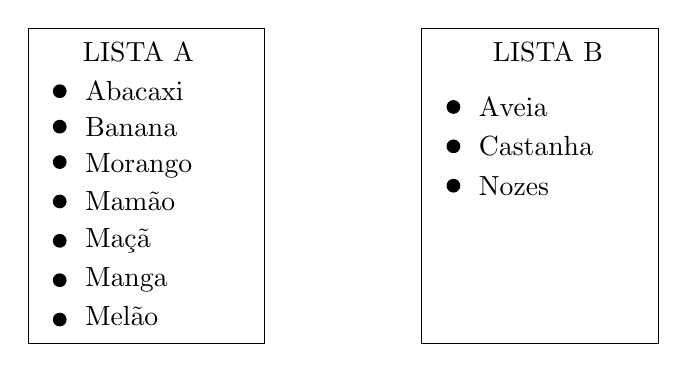
\begin{tikzpicture}
         \draw   (1,0) rectangle (4,4);
          \draw  (-1,0) rectangle (-4,4);
          \node at (-2.6,3.7) {LISTA A};
          \node at (2.6,3.7) {LISTA B};
          \draw (-3.6,3.2)[fill] circle [radius = .08];
          \node at (-3.4,3.2) [right]{Abacaxi};
          \draw (-3.6,.3) [fill] circle [radius = .08];
          \node at (-3.4,.35)[right] {Melão};
           \draw (-3.6,.8)[fill] circle [radius = .08];
            \node at (-3.4,.8)[right] {Manga};
           \draw (-3.6,1.3)[fill] circle [radius = .08];
            \node at (-3.4,1.3)[right] {Maçã};
           \draw (-3.6,1.8)[fill] circle [radius = .08];
            \node at (-3.4,1.8)[right] {Mamão};
           \draw (-3.6,2.3)[fill] circle [radius = .08];
            \node at (-3.4,2.25)[right] {Morango};
           \draw (-3.6,2.75)[fill] circle [radius = .08];
            \node at (-3.4,2.75)[right] {Banana};
            \draw (1.4,3)[fill] circle [radius = .08];
           \draw (1.4,2.5)[fill] circle [radius = .08]; 
            \draw (1.4,2)[fill] circle [radius = .08];
            \node at (1.6,3) [right] {Aveia};
            \node at (1.6,2.5) [right] {Castanha};
            \node at (1.6,2) [right] {Nozes};
            
        \end{tikzpicture}
    \end{center}
  Sabendo que esse paciente deverá escolher no mínimo 4 ingredientes da lista A e somente 2 ingredientes da lista B, o número de maneiras diferentes dele preparar essa salada de frutas é:
    \begin{enumerate} [(a)]
        \item 64
        \item 128
        \item 192
        \item 256
    \end{enumerate}
      \begin{sol}
       resposta: c \\
       no mínimo 4 ingredientes de A (4 ou 5 ou 6 ou 7) e 2 de B \\
       $\Longrightarrow (\mathrm{C}_{7,4}+\mathrm{C}_{7,5}+\mathrm{C}_{7,6}+\mathrm{C}_{7,7})\cdot\mathrm{C}_{3,2}=192$
      \end{sol}
  \end{ex}